\chapter{CMS Computing Model \label{sec:computing_model}}

\section{Introduction \label{sec:cms_computing_model:intro}}
\footnote{This review has largely been taken from~\cite{CMSNOTE_2004-031} and~\cite{CMS_TDR_PHYS_vol1}.} 
The extensive scope of the computing requirements at each LHC experiment were outlined in the previous chapter as was the need for CMS to develop its own computing infrastructure on top of the LCG. This chapter details the computing model chosen by CMS. 

The CMS computing model lists the 2010 requirements as 116.6 MSI2000~\cite{citeulike:847987}, 34\,PB of disk and 59\,PB of tape~\cite{CMSNOTE_2004-031}. In order to manage these resources effectively a highly developed and scalable computing model was needed. This model had to be capable of managing sufficient levels of resources while facilitating complex particle physics workflows for the non-expert user.

%The extensive nature of CMS's computing requiremernts was outlined n the previous chapter. This chapter refines tese requiremernts and describes the computing model chosen to satidfy these needs. CMS, like all the LHC experiments, with its large quantities of data and computational requirements, needs a highly developed and scalable computing model. By 2010 CMS requires 116.6MSI2000, 34700TB of disk and 59500TB of tape. A well designed management system is needed to make effective use of these resources.

Not all LCG institutions support CMS. Those that do include a large Tier-0 centre at CERN, 7 Tier-1's, $\sim$\,25 Tier-2's and many more Tier-3 centres. CMS also requires an analysis facility at CERN to be available for analysis activities close to the experiment, termed the CMS CERN Analysis Facility (CAF).  

%The nature of the challenge facing CMS computing is exactly the kind of problem the grid paradigm was designed to solve. CMS relies on LCG for its computing infratructure. The CMS grid hierarchy involves a large Tier-0 centre at CERN, 5-10 Tier-1's located at large national computing centres, more than 25 Tier-2's at regional computing centres and many smaller Tier-3 centres hosted by individual universities. CMS also expects a facility at CERN to be available for analysis activities close to the experiment, called the CMS CERN Analysis Facility (CAF).

%%%%%
%In addition to the data flowing from the detector there will be a large amount of Monte-Carlo (MC) simulated data. MC data are being generated before the detector is operational for detector and proof of concept studies and later during CMS operation for comparison with the real data. CMS requires similar amounts of simulated and real data, $\sim1.5x10^{9}$ events/year, this significantly adds to the storage and CPU requirements. In order to effectively utilize these data the CMS computing model includes sophisticated data and workload management systems. 
%%%%%

%%%%%
%%The scale of the problem facing the CMS computing system is vast, consisting of large amounts of data, distributed among multiple geographically separated centres, with hundreds of physicists around the world requiring access to any particular piece. This is the kind of problem that the grid paradigm was designed to solve. CMS follows the general grid architecture of a tiered hierarchy. This hierarchy is distributed geographically and is consistent with the nature of the CMS collaboration, thus allowing CMS to benefit from the resources and expertise which exists at these centres. The CMS grid hierarchy involves a large Tier-0 centre at CERN, 5-10 Tier-1's located at large national computing centres, more than 25 Tier-2's at regional computing centres and many Tier-3 centres hosted by individual universities. CMS also expects a facility to be available for analysis activities close to the experiment, called the CMS CERN Analysis Facility (CAF).
%%%%%

%%%%%
%The Tier-0 is a production facility, it will secure a copy of the detector data, perform first pass reconstruction and stream data to the Tier-1's. The Tier-1's securely store data received from the Tier-0 and perform reprocessing. The Tier-2's receive data from the Tier-1's and allow users to perform batch and interactive analysis. Tier-3 centres will not be part of CMS managed infrastructure and instead will provide resources to CMS on a best effort basis. The CMS CAF will be used for high turn around computing services.
%%%%%

It is likely that the first years of CMS running will be characterised by a poorly-understood beam and detector. As understanding of the beam and detector evolves frequent data reprocessing will be required. During this time LHC operation will be inconsistent and the data flow from the detector will be erratic. Even so there will be great pressure to discover new physics as rapidly as possible, which will require full resource utilisation and the ability to prioritise critical activities.

Due to the expected constraints it has been decided that the computing model, during the startup phase, should be simple, reliable and give the best possible environment for early physics discoveries. The baseline computing model emphasises:
\begin{itemize}
\item Fast and frequent reconstruction;
\item Streamed primary datasets, with distribution and processing driven by priorities;
\item Joint distribution of raw and reconstructed data, allowing wide distribution and direct comparisons;
\item Multiple compact data formats with multiple distributed copies; and
\item An effective and efficient bookkeeping system.
\end{itemize}
There are also plans for beyond-the-baseline architectures and services, which will be implemented once the experiment has stabilised and greater functionality is required. These are not discussed in this thesis.

CMS will operate a structured analysis environment with analysis groups focusing on well-defined objectives whose priority has been determined by the collaboration. Computing resources will be prioritised for different activities; policies at Tier-0 and Tier-1 centres will be set to meet analysis group requirements, whereas controls at Tier-2 and Tier-3 centres will be looser. These controls will be especially important at start-up when only limited resources may be available.

\section{Data Formats}
A canonical Tier-1 lacks the storage capacity for a complete copy of the raw data, so to maximise data availability more compact data formats are to be utilised. This will allow data to be made available for analysis at multiple sites. The formats (data tiers) used are:
\begin{itemize}
\item RAW. This is the output format of the HLT farm. It contains data from all detector channels as well as the Level 1 and High Level Trigger bits. The target event size is 1.5 MB;
\item RECO. This is the output from event reconstruction of the RAW data, where, objects (tracks, vertices etc.) have been reconstructed and calibrations applied. The target event size is 0.25 MB;
\item AOD (Analysis Object Data). This is the output from further reconstruction (reprocessing) of RECO data. Physical objects (electron, photons etc.) have been reconstructed and calibrations applied. This is expected to be the primary data used in analysis. The target event size is 0.05 MB; and
\item TAG. This format indexes other event data and is the output from skimming of event data. This process is used to identify events with similar characteristics. This format has not been implemented to date.
\end{itemize}
When data is collected/produced it is grouped with similar data into datasets. This grouping is driven by the HLT bits. The same dataset may have RAW, RECO and AOD data tiers, therefore both must be specified to identify data uniquely.

\section{Tier roles \& responsibilities}
CMS has assigned each tier within the LCG MONARC hierarchy roles according to their resource levels. The required computing resources at each Tier are listed in Table~\ref{fig:timeprofile}. 

\begin{table}[tbp]
  \centering
  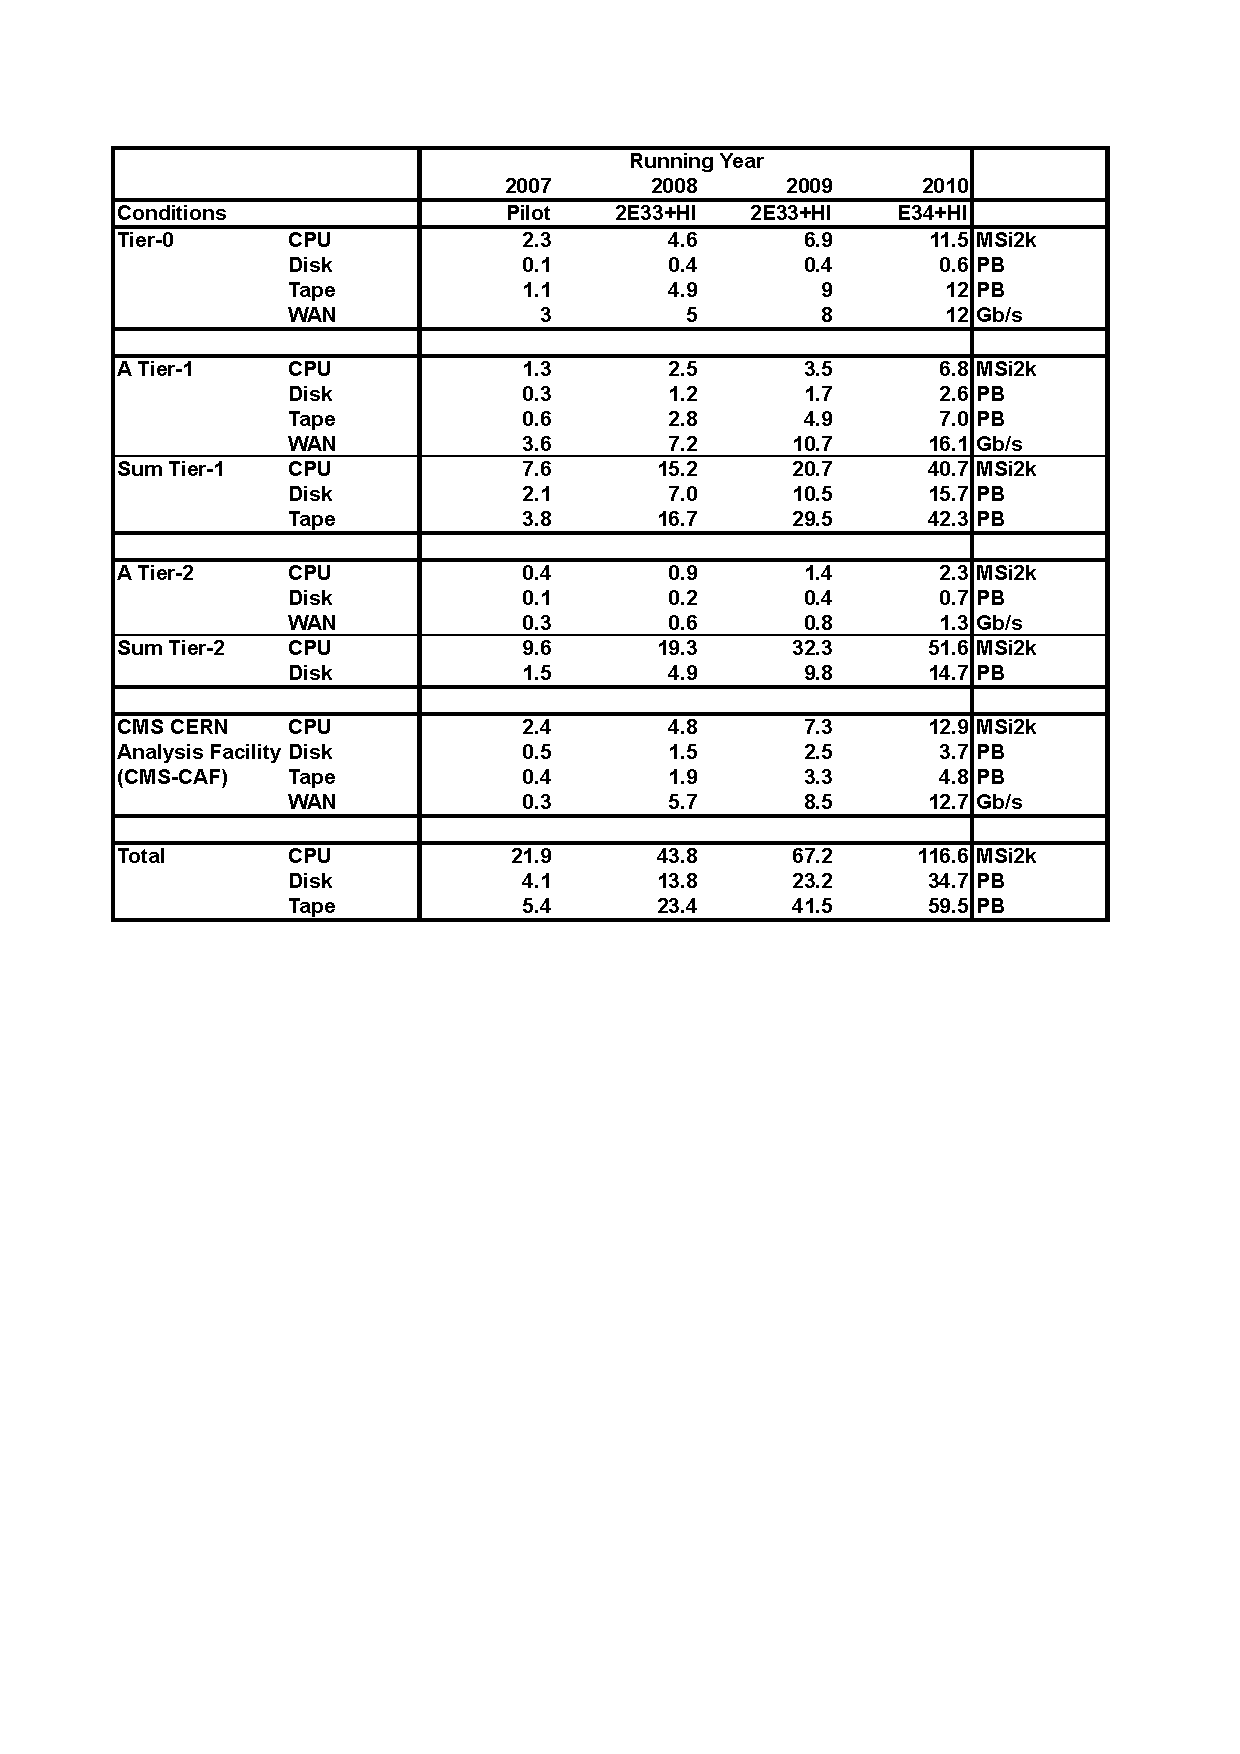
\includegraphics[width=0.88\linewidth]{cms_computing_model/timeprofile}
  \caption{Time Profile of CMS Computing Requirements.~\cite{CMS_TDR_PHYS_vol1} These requirements change frequently, see ~\cite{revised_resources} for up to date figures.
  \label{fig:timeprofile}}
\end{table}

\subsection{Tier-0}
The responsibility of the Tier-0 is to accept data from the CMS online system (HLT). This is then archived, reconstructed and a copy distributed to the Tier-1's. It is essential that this proceeds with minimum delay to avoid a build up of data on the input buffers. Thus the resources of the Tier-0 must be dedicated and continually available. During periods that CMS is not taking data the Tier-0 will be used for heavy-ion reconstruction, which takes $\sim$10-50 times more processing than that of a proton-proton event. %%Thus usage of the Tier-0 is expected to be continuous and is required on a 24/7 basis.

\subsection{Tier-1}
The Tier-1's have a number of responsibilities including secure data storage and centrally co-ordinated processing. The Tier-1's as a whole are responsible for storing the custodial copy of the RAW data with the Tier-0 copy only accessed in the event of data loss. Due to its small size each Tier-1 stores the entire AOD. Both real and Monte Carlo data is included in the Tier-1 storage.

Tier-1 data processing includes reprocessing, skimming and a small amount of analysis. A Tier-1 will reprocess all of its data at least twice a year. A limited amount of well managed analysis will be allowed, probably making use of the RAW data. All activity at the Tier-1 will be managed and subject to CMS control and policies.

\subsection{Tier-2}
The main role of the Tier-2 is to support a portion of the physics community and run analysis jobs. Many detector-specific calibration and analysis groups are expected to operate at a Tier-2 ``close'' to the relevant experts. It is expected that such a Tier-2 would provide extra resources for that group, i.e. extra storage space and relevant software installations. The analysis will originate from both local and remote users. 

A nominal Tier-2 has enough disk space (no tape is required at Tier-2's) to hold approximately one-tenth of the current RECO data and half of the current AOD. Tier-2's have no custodial responsibility for data. Data will be downloaded, analysed and periodically replaced. As well as providing for analysis the Tier-2's must provide processing capacity for Monte Carlo production ($\sim10^{8}$ events per year). These data will be stored at the Tier-1.

%%%%%
%A standard T2 is a single site with all resources located together, however there is another type of Tier-2 site, the federated Tier-2. This Tier-2 may be made of multiple institutions linked together and sharing resources. As long as the Tier-2 is presented to the user as a single entity with appropriate levels of resources the actual configuration of a Tier-2 is left to the local management.
%%%%%

\subsection{Tier-3}
In CMS, Tier-3 sites are users' home institutes, where they are provided with the facility to develop and submit their analysis. The major usage pattern consists of users submitting analysis jobs either to run locally or at a remote site and for the results to be returned to them at the Tier-3. Some Tier-2's will also provide Tier-3-type facilities as well as fulfilling their nominal role as defined by the computing model.

\subsection{CMS-CAF}
The CMS-CAF provides general facilities for the whole collaboration, serves users without a local Tier-1/2 and provides facilities for low latency, experiment-critical activities. General services include user logins, database support, production bookkeeping and software repositories. High priority work, generally taking advantage of the only copy of all RAW data, will include:
\begin{itemize}
\item Detector diagnostics - particularly useful during early running stages and after periodic shutdowns;
\item Trigger performance studies - i.e. optimisation and algorithm development. These studies will be carried out in response to changing understanding of the detector or the need to focus on specific channels; and
\item Calibration and alignment - to support the HLT and to be used in the (re-)reconstruction at the (Tier-1) Tier-0.
\end{itemize}

The analysis facilities offered to users will be approximately equivalent to 2 nominal Tier-2 centres. However, it is essential that individual users cannot interfere with the critical work undertaken here, hence strict policies and quotas will be put in place.

\section{Data Distribution}
The data distribution system must be capable of multiple simultaneous transfers between sites while maximising network usage and ensuring data integrity. Transfers must be automatic, provide for error recovery and conform to priorities determined by the experiment. It is vital that data from the detector be archived and streamed to the Tier-1's with minimum delay and without data loss. Lower priority transfers include data for user analysis being streamed to the Tier-2's. Monte Carlo data generated at the Tier-2/3's must also be moved to the Tier-1 for long-term storage.

The planned data flow for CMS is illustrated in Figure~\ref{fig:streams}. The online system will be set to write out events at the maximum rate that the offline computing model can support, which ties the physics reach of the experiment to the performance of the offline computing system. In the baseline model this rate will be set to a minimum of 225 MB/s giving an event rate of 150 Hz.

If an event passes the HLT it is passed to the offline system. The Tier-0 archives a copy of this data then passes it through a first pass reconstruction that results in RAW, RECO and AOD data products. 

Each Tier-1 receives a share of the RAW and RECO data consistent with their resources and a complete copy of the AOD. Periodically the Tier-1 will reconstruct its RAW data to produce new RECO data and then reprocess that to produce new AOD.

The Tier-2's obtain a share of the RECO data and half of the AOD from the Tier-1. The specific content will vary as physics priorities change and Tier-1 processing progresses. As such, a Tier-2 is expected to be capable of refreshing all of its data within 30 days, corresponding to a data import rate of 5 TB/day.

%datasets will be shared amongst the Tier-1's, which will periodically replace the RECO by performing re-reconstruction of the RAW data as understanding of the detector changes. 


%%%%%
%%For performance reasons events from the HLT are passed in one of $\sim$10 ``online'' streams. A copy is made of these streams and archived at the Tier-0. The online streams are then passed through a first pass reconstruction which results in $\sim$50 datasets containing RAW and RECO data. The reconstruction will initially be performed at the Tier-0 with the Tier-1's carrying out periodic re-reconstruction as understanding of the detector changes. The RAW + RECO datasets will be shared out amongst the Tier-1's with an additional copy archived at the Tier-0.
%%%%%
\begin{figure}[!tbp]
  \centering
  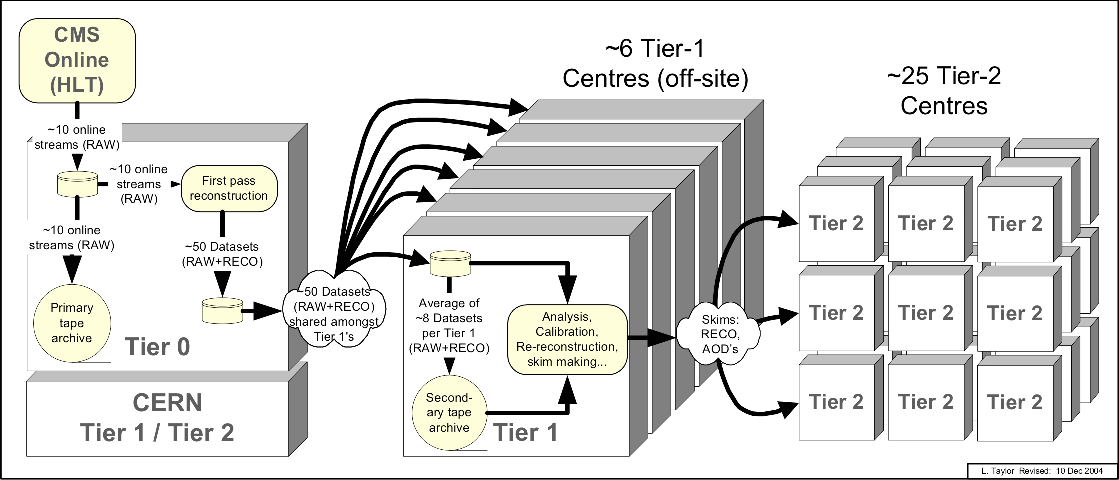
\includegraphics[width=1\linewidth]{cms_computing_model/cms-streams}
  \caption{Schematic flow of bulk (real) event data in the CMS Computing Model.
           Not all connections are shown, e.g. peer-to-peer connections between Tier-1's and Monte Carlo data transfer from the Tier-2 to Tier-1.~\cite{CMS_TDR_PHYS_vol1}
  \label{fig:streams}}
\end{figure}

%The Tier-2's obtain RECO data and half the AOD from the Tier-1 and send back generated Monte Carlo.

%The first copy of the AOD is be produced at the Tier-0 as an adjunct to the main first pass reconstruction step. The Tier-1's are then responsible for periodically reprocessing their RECO data to replace the existing AOD. The entire AOD is to be distributed to all Tier-1's as well as half to each Tier-2. Data flow to the Tier-2's will consist of both RECO and AOD datasets. With MC data flowing from the Tier-2 to Tier-1.



%\section{Examples of user activities}
%Here three potential use cases of the computing model are presented. They are taken from~\cite{CERN/LHCC-2005-023} and are intended to show how the computing model will satisfy the needs of the collaboration.

%\subsection{Mainstream analysis}
%A member of the Higgs Physics Group in 2009 is searching for the SUSY Higgs in a particular decay channel. The collaboration has judged this to be a high priority search and the group has been allocated resources at several Tier-2 centres to carry out their work. The Tier-2's made available to the members of the group will not always be the closest to a particular member. However it is likely that physicists in the same group will be allocated resources close together to allow shared usage of data and storage space.

%Periodically the group will ask for a modest amount of AOD or RECO data to be transferred to their Tier-2 to allow it to be analysed. If the data is not at their 'local' Tier-1 centre it will be copied to the Tier-1 and then to the Tier-2 transparently, possibly taking a few days. The group may put in a request for officially generated MC. Once accepted this request is scheduled centrally and constituent jobs are run at Tier-2 and Tier-3 centres around the world. The resulting events are copied to the local Tier-1 and Tier-2 centres. Here they are available to other members of the collaboration. 

%If the group requests a high priority analysis of data at multiple Tier-1 sites, and collaboration management approves, jobs will be scheduled at the relevant Tier-1's. If these jobs are given a higher priority than re-reconstruction which may already be running, the re-reconstruction jobs will be migrated to the Tier-0. If the group requires higher statistics they may request that Tier-1 centres skim events in the first pass AOD as they arrive, creating a new dataset. This new dataset may then be streamed to the Tier-2 where analysis may be performed on it.

%\subsection{Calibration study}
%A CMS physicist is a member of a group that is responsible for monitoring and calibration of the ECAL detector. In this role the group runs Data Quality Management (DQM) jobs to check that the prompt calibration system at the CMS-CAF is operating correctly. It is important that this system is operating correctly as the results are fed back to the first pass reconstruction within an hour of data taking. In order to monitor this process a sample of events are analysed from the reconstructed data. This is ensured by using a high priority but low statistics express stream which is analysed with low latency at the CMS-CAF.

%Due to a problem the calibration system fails over a period of a few days and the correct calibration constants are not used during first pass reconstruction. Before this problem is fixed the events are distributed to the Tier-1 centres. Since the ECAL calibration is critical for multiple analyses the collaboration decides to perform a second pass reconstruction on the affected events. This is performed at the Tier-1 centres with a high priority. 

%As a result the calibration group develop a new version of their algorithm but need access to a very large event sample to test it. They put in a request to the collaboration to run over a large amount of RAW data, this is approved with a medium priority, and their jobs run at the Tier-1 centres over the next few weeks. Once they are satisfied with the new algorithm it can replace the old one in the mainstream reconstruction.

%\subsection{Hot channel}
%A physicist is interested by a new GUT formalism that predicts a certain event signature and tries to look for it. The relevant group has limited resources and assigns this search a low priority. The physicist has access to resources at his local Tier-2 and uses them in his search, he requests a transfer of relevant AOD samples, this again is set at a low priority, and slowly the events are transferred. The physicist carries out his study and does indeed find the signature he is looking for, he contacts colleagues and ascertains that they to see the same signature on the same data at the Tier-2. Other members of the analysis group then begin to get interested and resources at the Tier-1 are assigned for a more thorough search in the RECO data. The interest becomes such that the centre becomes heavily loaded and therefore the events are replicated to another Tier-1 to make more resources available.

%The interest is so high in this work that the event signature is added to the express channel at the Tier-0 and analysis jobs run over the RECO data at the CMS-CAF as soon as possible. The result of all this interest is that a bug is found in the CMS trigger. This places a lot of physics results in doubt hence the impact must be determined quickly. Therefore the collaboration takes the decision to devote all available resources to reprocessing selected datasets. The computing policies are rapidly changed to accommodate this. As a result the first pass reconstruction is not carried out in real time instead the data is stored at the Tier-0 and Tier-1 for later reprocessing. This leaves capacity at both the Tier-0 and Tier-1 available for re-reconstruction. The Tier-2 centres are then used by selected physics groups to carry out their analyses. Once the reprocessing is complete the Tier-0 and Tier-1 centres resume normal operations with additional resources being scheduled at the Tier-1's for reprocessing until the backlog is under control.

%%%%%
%\section{MC production?}
%???
%%%%%

%%%%%
%\section{CMS policies}
%The CMS competing system is composed of a large number of semi-autonomous centres, operating with different policies and resources. These resources may be shared amongst multiple experiments and scientific disciplines. It is required that the resources allocated to, and used by, CMS be accounted for.
%
%It is the goal of the CMS computing system to allow maximum flexibility and freedom to its users. However this is likely to be offset by a high contention for resources, especially during the early running period. Therefore CMS requires the ability to set policies determining data placement and resource usage. These policies are expected to change rapidly as the collaborations priorities change. Any CMS user must be potentially able to use any CMS resources with a priority set by the collaboration.
%%%%%

\section{Computing Services}
CMS has developed the following guiding principles for its computing services:
\begin{itemize}
\item Optimise for read access. In general CMS data will follow the general HEP pattern of being created, never modified and subsequently read many times;
\item Optimise for the bulk case, while still allowing basic tasks. In CMS the large amounts of data and jobs will require operations on a large scale i.e. the data transfer will be managed at the dataset level. However the functionality still exists for users to copy individual files;
\item Minimise dependencies of processes on the worker nodes (WNs). CMS expects $10^{3} - 10^{4}$ worker nodes to be in constant use. This presents a large reliability problem as nodes fail or suffer outages. The WN is made more reliable by removing as many external dependencies as possible. Any dependencies that do remain should be local to a site to avoid any single point of failure for the entire system;
\item Allow provenance tracking. It is a requirement of the software and computing frameworks to track the provenance of datasets. This includes run-time parameter sets and software versions;
\item Site configuration information should remain local to the site. This allows system administrators to setup their site however they wish while allowing CMS applications to discover any information required; and
\item Keep the solution simple. The start-up of CMS is likely to be a hectic and confusing time, thus it has been decided that the computing system should be as simple as possible while providing all necessary functionality.
\end{itemize}

The CMS computing system consists of a distributed set of systems and services. These services consist of a mix of generic grid, site-specific and CMS-specific components. Figure~\ref{fig:comp_arch} shows the major components of the computing system. The main systems are:
\begin{itemize}
\item Data Management System - the CMS data management and movement tools.
\item Grid Workload Management System - the core grid systems and services of which CMS makes use.
%\item Other CMS specific services. 
\end{itemize}

\begin{figure}[!tbp]
  \centering
  \vbox{
    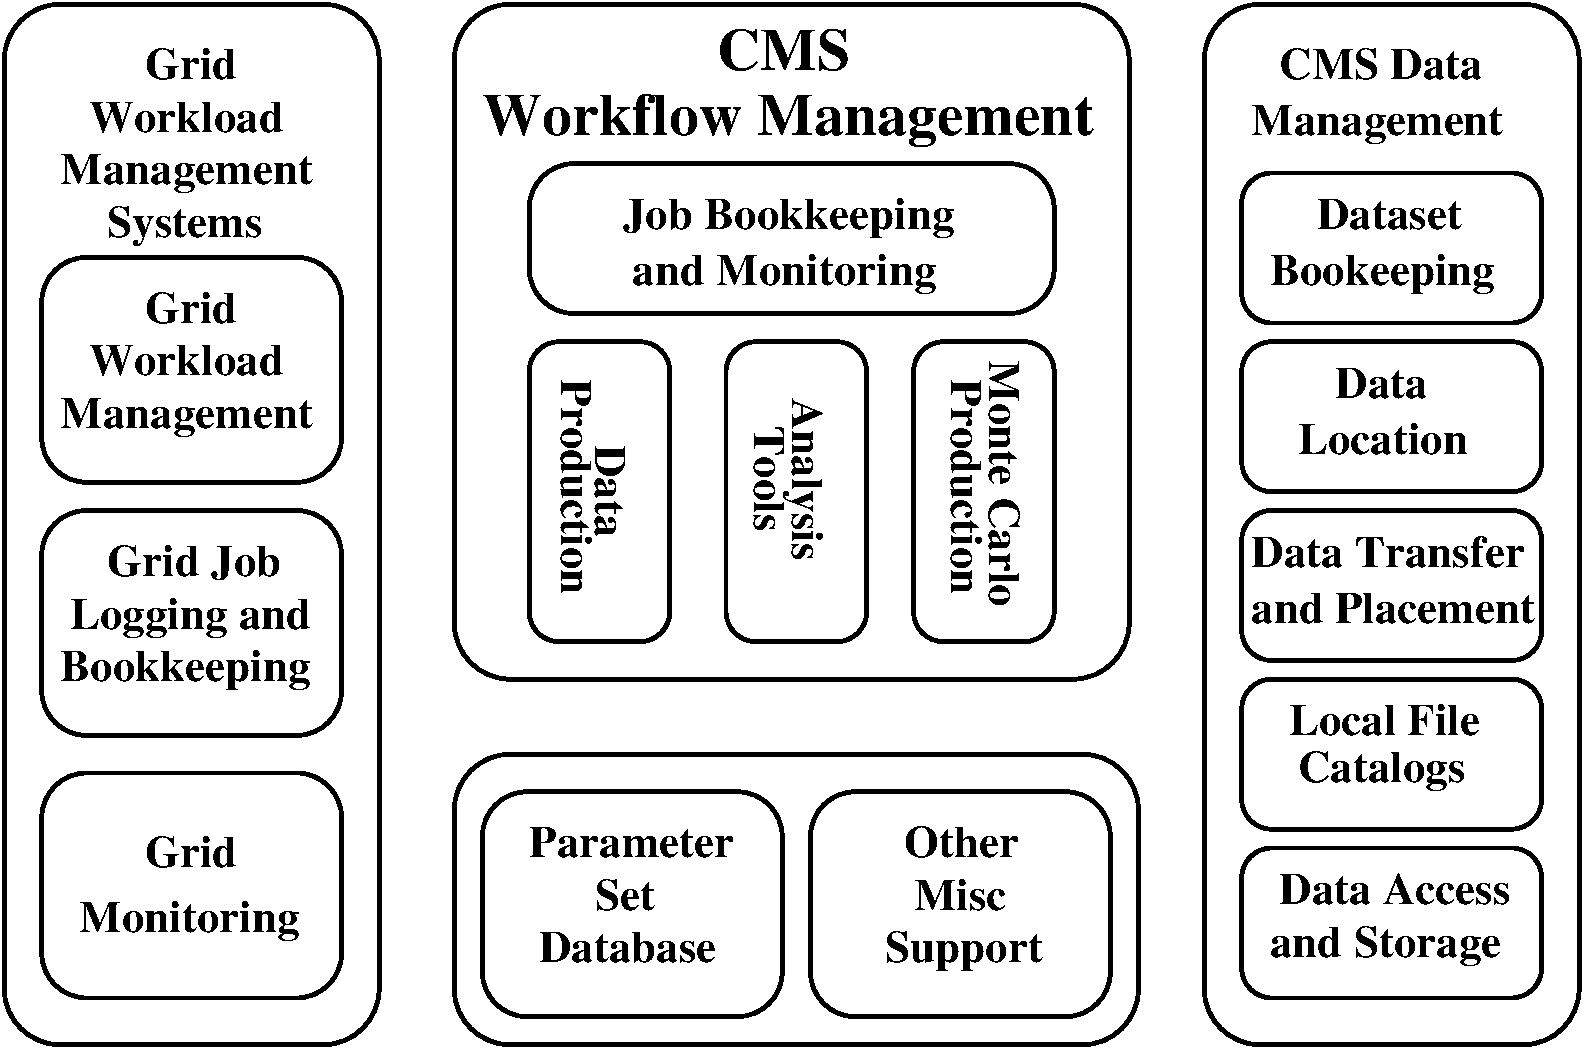
\includegraphics[width=0.95\linewidth]{cms_computing_model/global_architecture}\\[1mm]
    \caption{Overview of systems and services supporting the CMS workflow
           management system.~\cite{CMS_TDR_PHYS_vol1}
    \label{fig:comp_arch}}
  }
\end{figure}

These pieces are tied together by the CMS Workflow Management (WM) system. This system supports all necessary workflows in CMS, including (re-)reconstruction, reprocessing, calibration, MC production, skimming and user analysis, while shielding users from the complexity and implementation details of the underlying components. 

\section{Data Management System}
%\subsection{Introduction}
The CMS Data Management (DM) system is designed to provide necessary data management functionality for CMS, i.e. allowing physicists to discover, access and transfer various forms of data. These facilities will be used in situations ranging from organised large-scale data placement operations to individual user file transfers. The system must be suitable in all situations.

In the baseline model the experiment data placement will be pre-determined leaving the CMS WM system to steer jobs to the correct location. The DM system will provide functionality for the WM system to accomplish this. 

The Data Management system understands both user-oriented terms such as dataset as well as technical details such as file names that need not necessarily be exposed to the user. An ``event collection'' is defined as the smallest data unit that may be selected. A dataset is defined as a set of ``event collections'' that share a set of trigger bits. The dataset concept is used by physicists to specify data for their analysis jobs, but the jobs will be configured with, and at run time refer to, event collections. Event collections are stored in files that are themselves grouped into ``file blocks''. These file blocks are groups of files that are generally distributed and accessed together.

The DM architecture is based on a loosely-coupled set of components, which together provide the functionality required of the system. The basic components of the system are:
\begin{itemize}
\item Dataset Bookkeeping System (DBS) - lists the available data. For the physicist this will be the primary means of data discovery. The DBS can be queried with criteria such as run range, data tier, software version and data quality flags. Results will be returned as either datasets, event collections or file blocks. These can then be used to configure the CMS analysis framework;
\item Data Location Service (DLS) - maps file blocks to sites. Queries will result in a list of sites that contain the given data;
\item Data Placement and Transfer System - handles file transfers. The data placement system will be used to manage data movement and placement. File blocks will be subscribed to sites and the request passed on to the data transfer system. The data transfer system will handle reliable end-to-end transfers of individual files;
\item Local File Catalogue - provides file lookups at a site. This catalogue presents a POOL interface that is able to return file locations at a site and can be used by CMS applications to locate event data. In the current implementation this is a text file that contains lookup rules to determine the correct file location; and
\item Data Access and Storage System - provides access to files and manages the local mass storage system, if any.
\end{itemize}

%%%%%
%*FIXME* Wanted?
%The Data Management system handles many levels of complexity *FIXME* from the global bookkeeping of the experiment to the moving of files local to a site. CMS splits this into two ``scopes'': global and local. The global scope is taken to mean the system used by physicists to find which data is available. These services will run at the Tier-1 and Tier-2 and will have well defined contact points known to the collaboration. Local scope refers to data created and accessed by a sub-set of the collaboration, this includes ``private'' data and MC production that has not yet been published to the global scope. In the local scope not all the DM system components will be required. It may be possible to ``publish'' data from a local scope to the global one, this would allow users to create their own data, validate it and make it available to the collaboration.
%*FIXME*
%%%%%

%The Data management system supports user oriented terms such as dataset and technical details such as files. An ``event collection'' is defined as the smallest data unit that may be selected. A dataset is defined as a set of ``event collections'' that are naturally grouped together. The dataset concept is used by physicists to specify data for their analysis jobs however the jobs will be configured with, and at run time use, event collections. Below the view of event collections are physical files. In CMS the packaging of event collections into files will be done in such a way as to have an average file size of at least 1 GB, as mass storage systems have scaling issues with small files. CMS also defines the term ``file block''. This is a set of files that will generally be accessed and transferred together and is expected to be in the range 1-10 TB for data management reasons.

%\subsection{Dataset Bookkeeping System}
%The Dataset Bookkeeping system (DBS) provides a mechanism for querying the event data. For the physicist it is intended to be the primary means of ``data discovery''. The information returned from the DBS will be site independent. Typical operations are expected to involve selecting datasets and defining new datasets from selected events in other datasets. Datasets may be searched for using criteria such as run range, data tier, software version and data quality flags. Once selected a list of event collections are returned to allow analysis or production job configuration. Similarly the DBS will provide the mapping from event collections to files and file blocks. 

%%%%%
%The DBS also provides information about provenance tracking of collections such as the event collections it is derived from, software versions used during reprocessing and MC generation. The DBS may also contain summary information of the collections it holds, i.e. estimates on the integrated luminosity, information on the runs including possible data quality flags. The DBS will not track job bookkeeping, MC requests etc. these will be stored by the WM/Production bookkeeping systems.
%%%%%

%%%%%
%It is expected that the DBS will be available in several forms. The global scope will be satisfied by an instance at CERN with mirrored copies at other locations to aid access. It is also possible that a DBS may be in use at an institute with local scope, containing details about private data. The DBS is a VO specific service that describes CMS data in terms of datasets and data blocks and so will be constructed by CMS on top of grid services.
%%%%%

%\subsection{Data Location Service}
%The Data Location Service (DLS) is used to find out where instances of data exist. This maps file blocks to storage elements. It is likely that the DLS will be implemented as a two tier system, a local DLS instance will publish the data-blocks available and a global instance aggregates the information from the local instances. Queries to the global DLS will result in a list of sites that contain a given data-block.

%The file catalogues are expected to provide file attributes such as file size and checksums but will not contain any CMS specific attributes. The catalogue is expected to be highly scalable and to be as robust and reliable as the data storage.

%\subsection{Data Placement and Transfer System}
%The data placement system is used to define, execute and monitor CMS policies on where data is to be located. This layer manages the allocation and release of storage resources and data transfers at the dataset level. The data transfer system handles reliable background transfers of files from multiple sources to multiple destinations at maximum data rates. 
%The data placement and transfers systems are implemented by the PhEDEx project. *FIXME* REF

%%%%%
%The requirements on such a system include a managed and structured data flows, multiple transfer modes and priorities. The CMS data flow is highly structured with data flowing from the Tier-0 through the Tier-1's to the Tier-2's. This kind of data flow is required as the Tier-0 could not cope with all sites connecting directly to it. The system must be able to track file transfers as they move through the different tiers and know when the data has reached its final destination and be able to release any temporary copies used during the transfer.
%%%%%

%Data transfers need to occur in different modes, the Tier-0 will push data out to the Tier-1's continuously, but must dynamically re-route data if one of them becomes unavailable. Tier-2 sites will want to subscribe to datasets that interest local physicists and here the data is pulled from the Tier-1's. All of these transfers must take place with the appropriate priorities set, obviously data streamed from the Tier-0 should be moved with a higher priority than a request from a Tier-2.

%The data placement service keeps track of file-blocks and subscriptions. A subscription request specifies the data to be transferred, the priority and whether the resulting copy should be considered as the custodial one (i.e. in the case of MC data transferring form a Tier-2 to Tier-1.

%The data transfer system operates at the file level, it receives assignments from the data placement system. It then handles the end to end transfer reliably using one of a group of tools depending on individual site configuration.

%\subsection{Local File Catalogue}
%The DLS provides the site and storage element that hosts an event collection but not individual file locations. The physical location of files is only known within a site by the local file catalogue. This catalogue presents a POOL interface which is able to return the physical location of a file based on it's logical file name or GUID. CMS applications only know about logical files and rely on the file catalogue to locate them.

%\subsection{Data Access and Storage Systems}
%The data transfer system in CMS expects an SRM interface to the mass storage system. This interface allows for file transfers, space allocation and deletions. Larger sites will be expected to provide secure storage, probably tape based, with large disk caches to allow applications to access the files. CMS applications require POSIX-like~\cite{citeulike:363700} file access.

\section{CMS Workflow Management System}
\subsection{Introduction}
The CMS Workflow Management (CMS WM) System combines the CMS DM and grid workload management systems and presents them in a uniform manner to the user. The WM system includes applications designed to support all major CMS workflows including prompt reconstruction, prompt calibration, re-reconstruction, reprocessing, calibration, Monte Carlo production and analysis.

The primary unit of work in the WM system is a task. The task contains an application, configuration parameters and optionally a data selection. The DBS and DLS search for the data selection and once the WM system discovers the nature of the data to run over, i.e. number of runs/events, it can decide how best to run the workflow. In general, the task will be split into many jobs each running over a subset of the total requested data. Once the individual jobs have been created they are submitted to a supported grid WMS. This then takes responsibility for scheduling the job at an appropriate site, i.e. one that contains the required data. Once the job is finished the CMS WM system will retrieve the results and handle any output files. 

Figure~\ref{fig:WM_general} shows how the CMS DM system and the grid WMS are combined. The UI is the gateway to both the grid and CMS WM system with both CMS WM applications and grid tools installed. Individual CEs and SEs in supported grid middlewares advertise themselves via their native information services. The CMS WM system can then run a given workflow on the most appropriate resources on any supported grid middleware. 

\begin{figure}[tbp]
  \centering
  \vbox{
  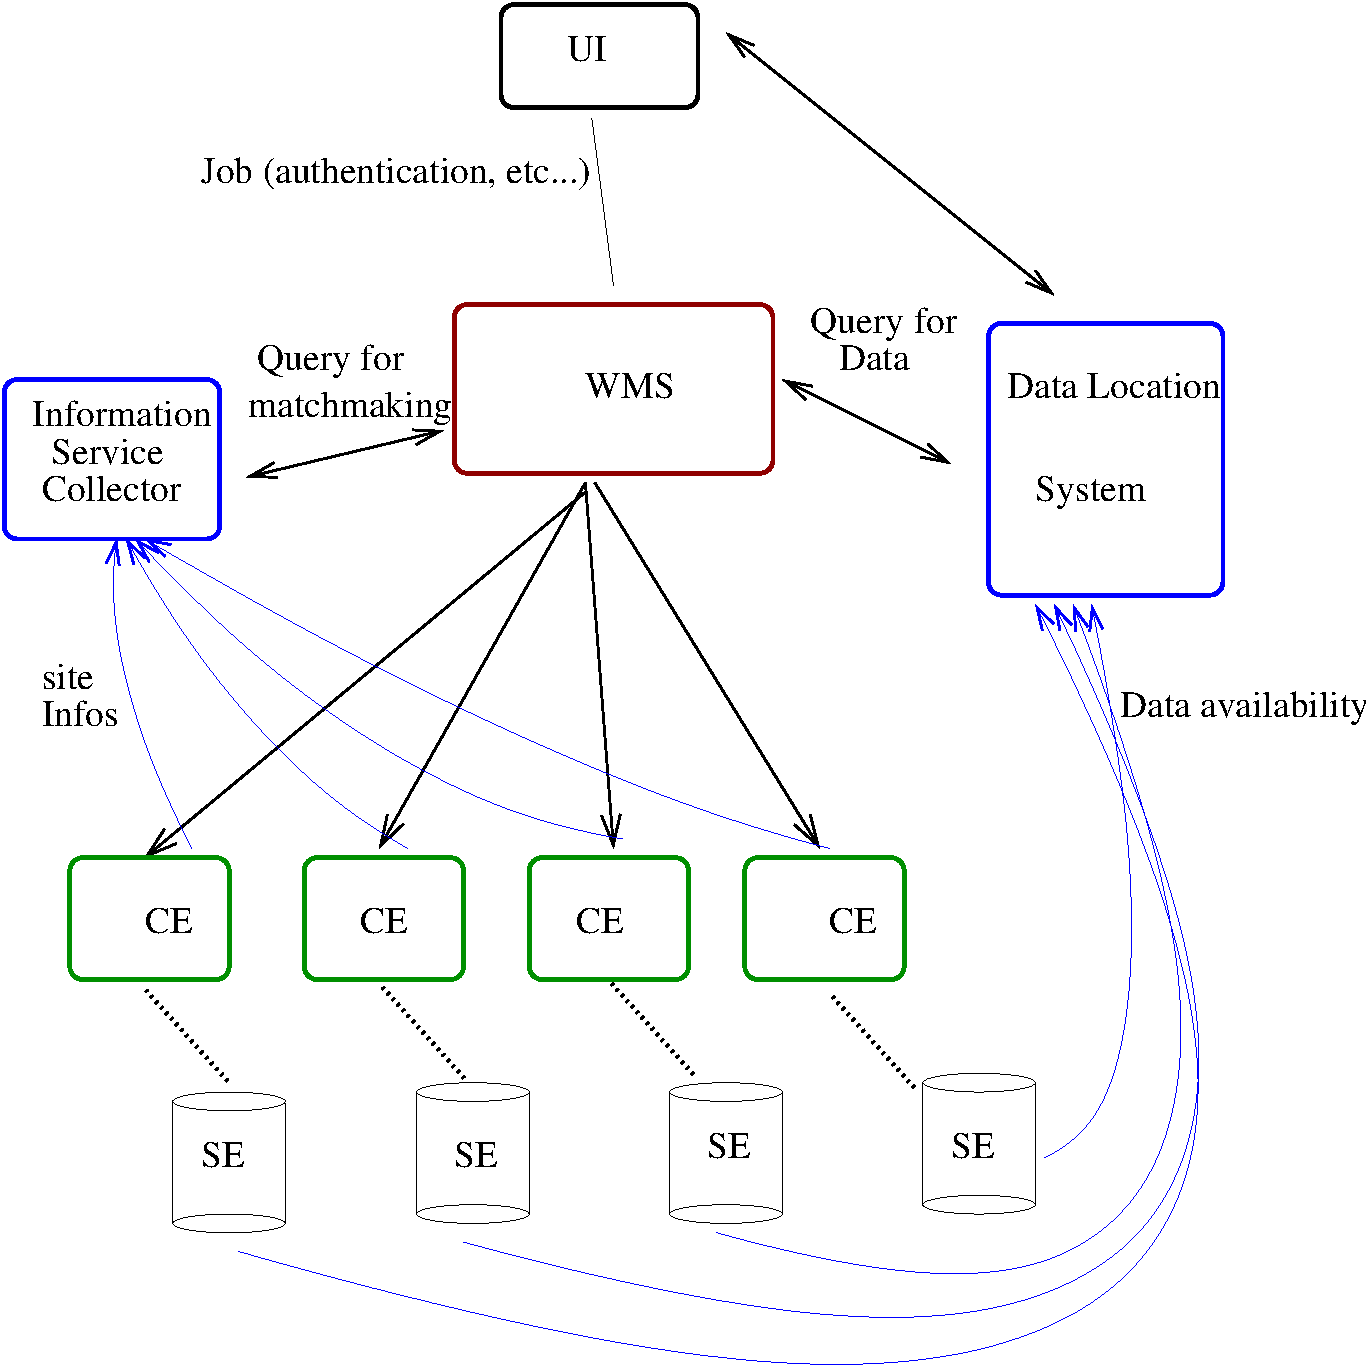
\includegraphics[width=0.65\linewidth]{cms_computing_model/Grid_WMS_base}
  \caption{The baseline CMS WM system architecture.~\cite{CMS_TDR_PHYS_vol1}
  \label{fig:WM_general}}
  }
\end{figure}

The work of the CMS WM system is simplified for workflows that run exclusively on the Tier-0 (prompt calibration and reconstruction) as no grid middleware is needed. 

\subsection{User analysis}
One of the prime supported CMS workflows is that of user analysis. These analyses are carried out by individuals or groups of physicists and will be the source of physics discovery at CMS. All data taken by CMS will be analysed many times by different groups, each looking for different physics. Classic CMS analysis, described below, limits the user to running over local data and requires the user to handle job creation, submission and output file handling. The CMS WM expands on this by providing full automation from analysis creation through to job splitting and output file handling.

%The CMS WM system (see Figure~\ref{fig:WM_analysis}) will provide a common interface to all grid implementations. For user analysis the CMS WM system takes a users analysis task and uses the grid infrastructure to submit it as multiple batch jobs to appropriate sites, i.e. ones that hosts the required data. Functionality includes data verification, site location, job splitting, packaging, submission and output retrieval. The CMS WM system is capable of interfacing to multiple types of batch system, both local and grid.


\subsubsection{Classic CMS Data Analysis}
Analysis of event data is performed with the CMS analysis framework. This provides a layer of common functionality (event access, reconstruction algorithms, calibrations etc.) that users may call on in their analysis programs. Users build their code against this framework and an executable is produced. This executable dynamically links with the framework libraries as extra functionality is required. User options, datasets and other parameters are passed via a configuration file. In CMS the standard practice is for the user's analysis code to produce an ntuple file that is then analysed with ROOT~\cite{citeulike:363715}, or similar a tool, to produce final plots.

The framework utilises POOL for file IO and catalogue functionality. The CMS analysis framework refers to data files via their LFNs and relies on POOL for file location and IO. This means that to run in the framework, the user has to specify, in their configuration file, at least one POOL catalogue that contains the required event files. The framework has no knowledge of the grid as it runs locally and assumes that files in the POOL catalogue are accessible. Users can only therefore analyse data at their local site, which is clearly incompatible with CMS's distributed data model. The CMS Workflow Management System solves this problem and provides the user with access to all CMS data and computing resources.

\subsubsection{Distributed User Analysis Workflow}
The classic analysis scenario is useful for developing analysis code and analysing small numbers of events. However most CMS analyses require running over thousands or millions of events. To do this a user has to write their own machinery to create possibly hundreds of analysis jobs then submit them and finally handle the hundreds of resulting output files. This process is tedious and prone to error.

A main function of the CMS WM system is to simplify and automate these functions for the user. Functionality includes data verification, data location, job splitting, packaging, submission, output retrieval and merging. This workflow is illustrated in Figure~\ref{fig:WM_analysis} and presented below.

\begin{figure}[tbp]
  \centering
  \vbox{
  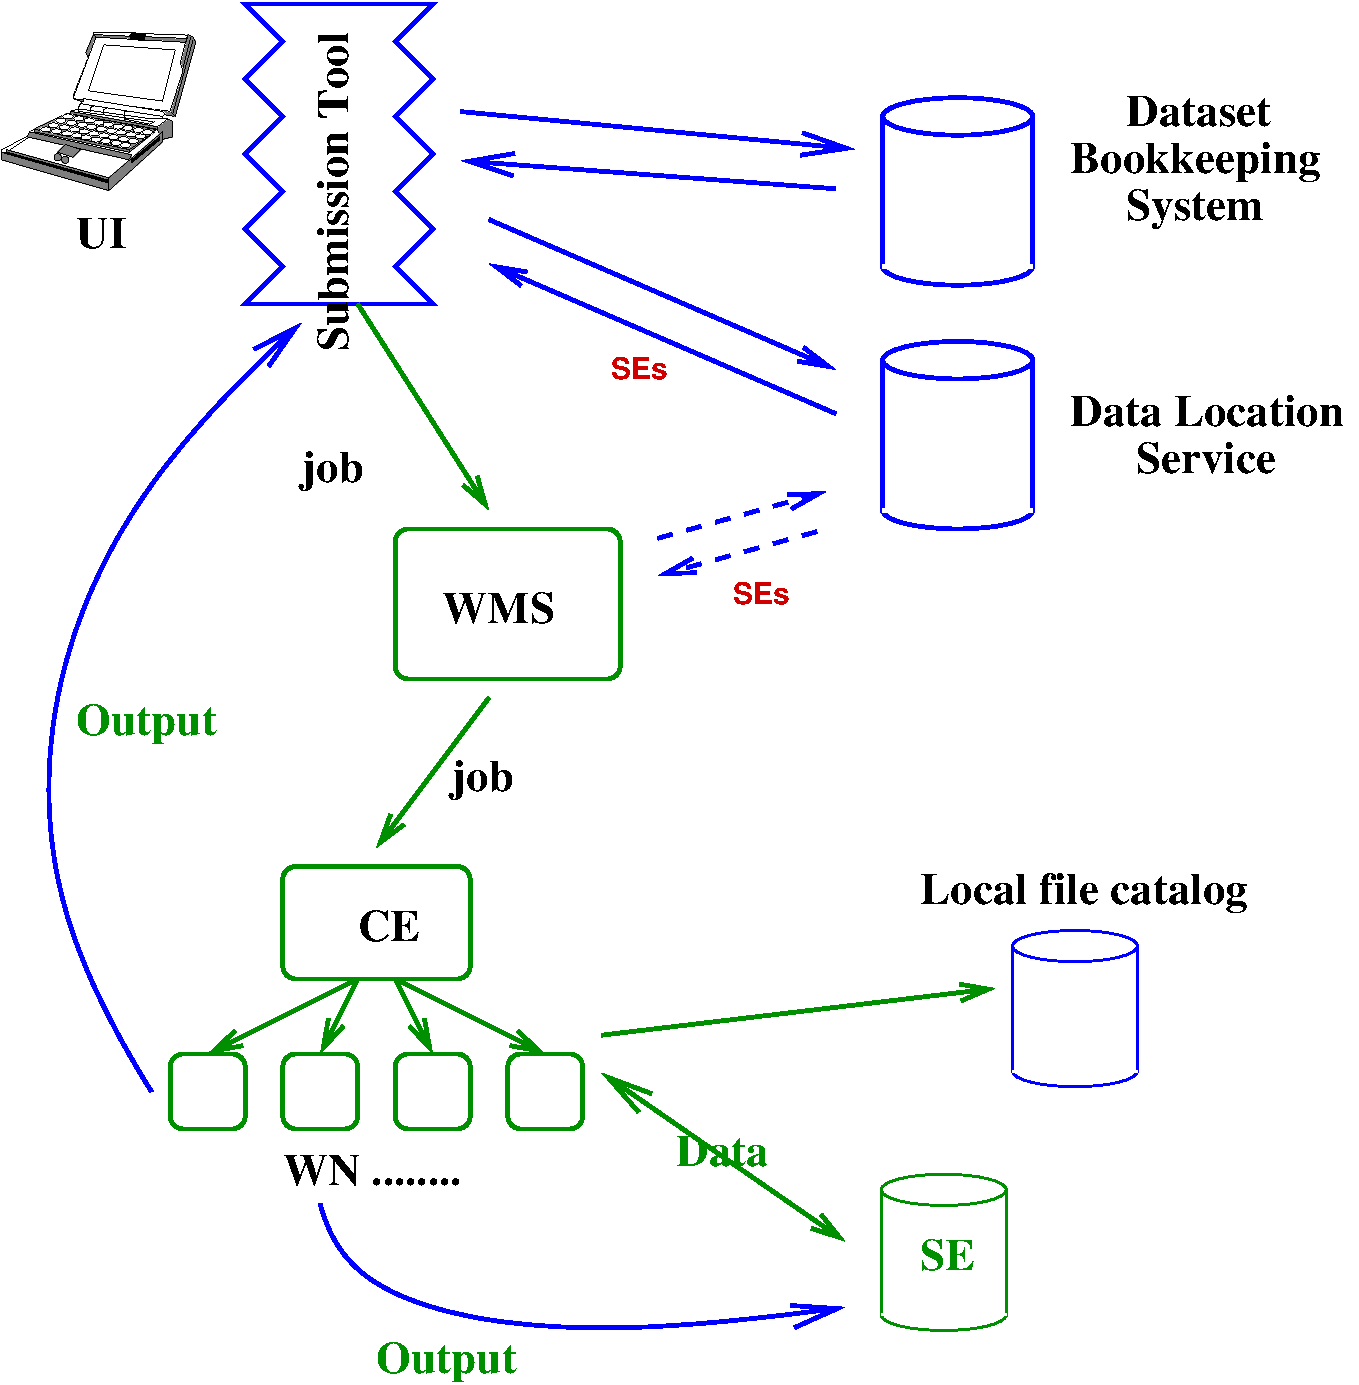
\includegraphics[width=0.65\linewidth]{cms_computing_model/WM_analysis}\\[1mm]
  \caption{Distributed data analysis with the CMS WM system.~\cite{CMS_TDR_PHYS_vol1}
  \label{fig:WM_analysis}}
  }
\end{figure}

%A major function of the CMS WM system is to manage user analysis. It takes a users analysis   For user analysis the CMS WM system takes a users analysis task and uses the grid infrastructure to submit it as multiple batch jobs to appropriate sites, i.e. ones that hosts the required data. Functionality includes data verification, site location, job splitting, packaging, submission and output retrieval. The CMS WM system is capable of interfacing to multiple types of batch system, both local and grid.

%A main function of the CMS WM system is to transform a user analysis task into a set of jobs to be run on the distributed computing system and to manage and log the relevant details. Here a typical user analysis workflow is presented.

The user begins (as in the ``classic case'') with an analysis application they wish to run, various configuration options and the data they wish to run over. These data may either be a named dataset or determined from a list of requirements i.e. software versions and HLT flags. The DBS is then contacted and the required data determined. This query results in a list of available event collections (and file blocks). The WM tool is then able to decide how best to divide up the user's analysis task into multiple jobs, each of which accesses a subset of the total data. The job splitting is driven by the user's configuration (maximum events per job, desired job run time etc.). 

The CMS WM system can then create the configuration for the jobs. This is a two step process as each job is configured at the CMS application level and at the grid WMS level. The application configuration requires the input event collections. The grid WMS configuration needs information in order to steer the job to a site that holds the appropriate event collections. This is accomplished by contacting the DLS to discover which storage elements (SEs) contain the required data. The user may specify that the output be returned directly to them or, if the output is likely to be large or accessed by others, copied to a remote storage element.

%%%%%
%The CMS WM system is now able to submit the users jobs. Until interoperability between the different grid WMS has been achieved the decision of which grid to use must be taken at submission time. Using the DLS the CMS WM tool can determine which grids have access to the data, if only one of them does then the decision about which grid to submit to is trivial. If more than one does the users preferences may be taken into account. When interoperability between grids is achieved the jobs will be submitted to a general service capable of steering their job to whichever grid is most suitable.
%%%%%

The CMS WM system submits, and tracks jobs to the WMS, or local site batch system. Jobs submitted to distributed resources are sent with a list of SEs that contain the requested data blocks and it is the task of the grid WMS to steer the job to the ``best'' site in terms of load, data access cost etc.

Once a job arrives at a site and locates the site-specific information, the user's application is presented with an environment that is identical to the development setup. This includes such things as CMS software installations and access to the CMS conditions DB. Once all of these have been found, the user's application runs exactly as during development with files streamed from the local storage system by use of the local file catalogue.

The user tracks their jobs using the CMS WM job logging and bookkeeping system, which uses the WMS information services as an information source. Optional real-time monitoring allows the user to monitor the progress of the job including such information as event number and CPU usage. This is optional as it requires the site to allow information to be sent from the job to an external service. The user may also find this unnecessary, especially if they have a large number of active jobs. Once the job finishes the output is either saved to an SE or returned via the WMS to the user's filesystem. The output from many jobs may be merged to aid the users further analysis of it.

%Output from the jobs is either made available for download to the users filesystem or accumulates on a predetermined SE. The SE will generally be used if the output is expected to be large or if it is to be shared among many users. 

%This is the baseline workflow for a user analysis task.

%%%%%
%As with AliEn Dirac mainly focusses on MC production with a prototype analysis component. Differences between DIRAC and LCG include pilot jobs and a pull rather than push model. By using Pilot jobs users submit jobs to the DIRAC system rather than submitting them directly to the underlying grid infrastructure. This allows the DIRAC system to take responsibility for the job and hide any inefficiencies of the grid. DIRAC makes use of sites where its custom agents have been installed and LCG through an interface that represents LCG as a single (large) site. Each of these sites can pull a job from the DIRAC production service when they have a free batch slot, by utilising this pull method there is maximum usage of computing resources. Should a site fail to complete the job, i.e. job crashes or service interuptions, DIRAC makes the job available to other sites. This avoids one of the sources of problems in LCG, manual job resubmission. In the LCG **"adaptor"** pilot jobs are sent out as regular grid jobs once these land on worker nodes they contact the DIRAc server and retrieve an appropriate job.
%%%%%

\section{Alternative computing models within HEP}
Within HEP the computing requirements of experiments vary considerably. Until recently all computing models relied on largely centralised resources. However the larger experiments are now restructuring their models to take advantage of grid computing.

\subsection{Tevatron Experiments}
The highest energy collider currently in operation is the Tevatron, based at Fermilab. The experiments based here (CDF~\cite{cdf} and D0~\cite{d0}) have some of the most demanding computing requirements of any HEP experiment to date. Together they require $\sim7$\,PB of tape storage by 2007~\cite{run2_comp_review}. Initially the computing models for both experiments relied on centralised resources with large computing farms at Fermilab. However, both are now taking advantage of significant computing resources outside of Fermilab. 
%Both are now utilising distributed resources, with CDF focusing on analysis and D0 on MC production. 
%Each experiment utilises resources at $\sim$20 remote sites. Currently 35\% of CDF analysis resources are available at remote centres and 10\% of D0 analyses are run at remote sites, ref chep04 Run2 computing.
% These shares are forecast to increase by 50\% by Dec 04 (look for current numbers). 
%FIXME change currently to as of 2005/06 etc. D0 MC numbers?

To facilitate this move to distributed computing Fermilab has developed some common grid services. Sequential Access via Metadata (SAM) is a data handling system that provides a mechanism for accessing distributed data. Data is transparently copied from remote sites on demand. The JIM (Job and Information Monitoring) services provide a mechanism for submitting SAM jobs to remote resources and then monitoring these jobs. The combination of SAM and JIM (termed SAMgrid) provides users with access to all available data and computing resources. Currently D0 uses SAMgrid while CDF uses SAM but not JIM, its submission software handles job submission via Condor and LCG tools.

Both experiments have significantly expanded their available resources by using distributed resources. Around 45\% of CDF's analysis capacity is located at remote sites and all D0's reprocessing and Monte Carlo generation has been completed offsite, as in the CMS computing model~\cite{run2_comp_review}. Both experiments are actively looking for ways to meet as much of their processing needs as possible remotely. Fermilab has developed their own grid technologies rather than join the LCG project, although a new project has been created aimed at allowing LCG and SAMgrid to interoperate.
%an interoperability project has been started to allow European and American resources to work together.

%The Tevatron experiments have included support for distributed resource utilisation when it became clear that significant resources were available. This support has only recently been implemented and each experiment is ramping up usage as the advantages become clear. differences to LCG? reasons?

\subsection{LHC experiments}
The computing models of the LHC experiments (ALICE, ATLAS, CMS and LHCb) were all designed after the development of the grid paradigm and therefore all utilise distributed computing. Each experiment's computing requirements were similar resulting in comparable computing models. The LCG project was specifically designed to provide a common grid layer for the LHC experiments, although each experiment makes use of it in a slightly different way.

ATLAS and CMS, the two general-purpose detectors, have similar computational requirements~\cite{LCG_TDR}. For planning purposes it is often assumed that these are equal but there are significant differences. An example of this is the amount of simulated MC data required; ATLAS will produce MC data equivalent to 20\% of their accumulated real data whereas CMS requires a ratio of 100\%. Another difference between the two is created by the composition of the two collaborations, which has resulted in more Tier-1 sites available to ATLAS than to CMS. To compensate for this CMS will rely heavily on resources at CERN (Tier-0 and CMS CAF) and the Tier-2's. The activities planned by each experiment for each Tier are similar with both models using the Tier-1's for re-reconstruction, reprocessing and skimming while the Tier-2's are responsible for user analysis and MC production.

ATLAS and CMS are also similar in their use of LCG software. Both have taken the WMS as given and written client-facing software that wraps and aggregates the LCG commands to provide higher level functionality and greater ease of use~\cite{citeulike:876380, citeulike:912507}. For data management both experiments found LCG tools lacking in high level management functionality and therefore created their own systems that managed data flows between sites using the LCG tools~\cite{citeulike:912497, citeulike:912501}.

ALICE specialises in heavy ion physics, where events are more complex than proton - proton interactions but run at a much lower luminosity. By 2010 ALICE requires approximately half of the processing power and a third of the mass storage of CMS~\cite{LCG_TDR}. The computing model, built to satisfy these needs, is very similar to the model used by ATLAS and CMS. Both have similar usage patterns at each of the tiers, the main difference being the scale of the activity.

In contrast to ATLAS and CMS the ALICE collaboration have created their own distributed computing framework, known as AliEn (Alice Environment)~\cite{citeulike:912514}. AliEn was developed at the same time as the LCG and was designed to provide transparent access to ALICE's homogeneous distributed resources. AliEn runs on ALICE resources and consists of central and site agents interfacing via SOAP web services.

%The job of AliEn is to present transparent access to homogeneous distributed resources. AliEn was designed to run on ALICE resources and consists of central and remote agents interfacing via SOAP web services. ATLAS and CMS used the RB for all WMS functions they simply wrote client facing software to wrap the low level LCG tools. AliEn by contrast was developed at the same time as LCG and was designed to provide transparent access to ALICE's homogeneous distributed resources

For workload management the main difference between AliEn and the LCG is that AliEn has a single task queue for all jobs whereas LCG has multiple RBs each managing jobs independently. Another difference between the two is the method used to distribute jobs; LCG uses the ``push'' method where ALiEn uses the  ``pull'' method. In AliEn, when a job slot becomes free at a site, a local agent contacts the central AliEn task queue and obtains a suitable job. In LCG the RB assigns jobs to sites according to the load in the system. There are advantages and disadvantages to each approach, e.g. multiple RBs have no single point of failure and can perform load balancing over the entire grid whereas a global job queue enables experiment-wide scheduling policies to be enforced. 
%Later versions of LCG and gLite will allow for both ``push'' and ``pull''.

Sites are reluctant to run VO-specific services due to the arbitrary hardware required, high levels of support and security concerns. Thus LCG looked for a way to normalise these services and developed the VO box concept. This was a grid node that was designed to run VO specific services for a site with remote management. Thus the site only needed to provide a standard grid node and each VO could organise their own services. These were used by ALICE to run the AliEn site services and were required at both Tier-1 and 2. However a number of Tier-2's were reluctant to run VO boxes and thus did not fully support ALICE.

%As sites increasingly move to adopting a uniform grid middleware layer (LCG, AliEn etc.) they are becoming unwilling to run VO specific services and agents. Therefore AliEn has been adapted to allow agents to act for an entire grid of resources. This agent pulls appropriate AliEn jobs from the task queue and submits them to that particular grids WMS. These grids appear as large individual sites within the AliEn system. AliEn has been so successful that the LCG successor, gLite, is partially based upon it.

LHCb specialises in B physics. LHCb's computing requirements are relatively modest: by 2010 it requires approximately a sixth of the processing power and a fifth of the mass storage of CMS~\cite{LCG_TDR}. LHCb has adopted a computing model substantially different from that of the other experiments. Due to the relatively modest processing requirements needed for reconstruction, reprocessing and skimming, enough capacity will remain at the Tier-1's for all analysis activity. This is in contrast to the other experiments where only limited, managed, analysis will be permitted on the Tier-1's. This has the advantages that only $\sim$6 sites are required to provide facilities for analysis, massively reducing the management overhead and Tier-1 to Tier-2 network traffic. However, user analysis is seen as a source of chaotic behaviour that must be effectively controlled otherwise it may interfere with the high priority managed workflows. The only role for Tier-2 and Tier-3 LHCb sites is MC production thus the level of storage required at these sites is low.

To implement their computing model LHCb have created their own framework, known as DIRAC (Distributed Infrastructure with Remote Agent Control)~\cite{citeulike:912522}. DIRAC consists of remote agents communicating via the XML-RPC protocol. A typical DIRAC workflow is similar to the approach of AliEn, with agents at each site pulling in jobs from a central task queue. To integrate with other grid middleware implementations, e.g. LCG,  DIRAC has developed the ``pilot'' job. A central agent exists that submits jobs to each grid's native WMS that, when executed, contacts the DIRAC task queue and obtains the real user's job. 
%This allows the ``pull'' paradigm to be used in grids which only implement the ``push'' model.

All of the LHC experiments rely on distributed computing. The more computationally intensive experiments (ALICE, ATLAS and CMS) have all adopted similar computing models. Reprocessing, skimming and limited analysis will be performed at the Tier-1's with the majority of user analysis conducted at the Tier-2's. All Monte Carlo (MC) will be generated at the Tier-2/3's. LHCb, due to its relatively modest requirements can handle all its non Monte Carlo processing at the Tier-1's. This greatly simplifies the system but the resulting effect on the Tier-1's is not fully understood. 

Both ATLAS and CMS rely on LCG to provide basic grid functionality with their custom applications handling the complex workflows. Both ALICE and LHCb have developed their own grid middleware layers. LHCb is integrating their software into LCG while ALICE is keeping a large fraction of their custom grid software.

\section{Summary}
The scale and complexity of CMS computing required a well designed computing model. This model is based on the LCG and provides increased functionality and ease of use. This functionality is divided into two main components: the Data and Workflow Management systems. One of the prime aims of the Workflow Management system is to support distributed user analysis. This is a complex application that had to bridge many systems and as such a number of prototypes have been developed. One of these is described in the next chapter.
